\documentclass[10pt, a4paper]{scrartcl}

\usepackage{vorschule}
\usepackage[
    typ=ab,
    fach=Informatik,
    lerngruppe={EF},
    nummer={I.3},
    module={Symbole,Lizenzen},
    seitenzahlen=keine,
    farbig,
    lizenz=cc-by-nc-sa-4,
]{schule}

\usepackage[
	kuerzel=Ngb,
	reihe={Informationen, Daten und Codierung},
	version={2020-09-7},
]{ngbschule}

\author{J. Neugebauer}
\title{Fehlerkorrigierende Codes}
\date{\Heute}

\setzeAufgabentemplate{ngbnormal}

\usepackage{qrcode}

\usetikzlibrary{matrix}
\tikzstyle{card deck}=[scale=.8,every node/.style={transform shape}]
\tikzstyle{card}=[draw,fill=gray!10,rectangle,rounded corners=1mm,minimum width=4mm,minimum height=7mm,anchor=south west]
\tikzstyle{white card}=[card,fill=white]
\tikzstyle{black card}=[card,fill=black]
\tikzstyle{card bg}=[fill=black!30]


\begin{document}

\ReiheTitel

\begin{wrapfig}
\begin{wrapfigure}{r}{4cm}
% field 1
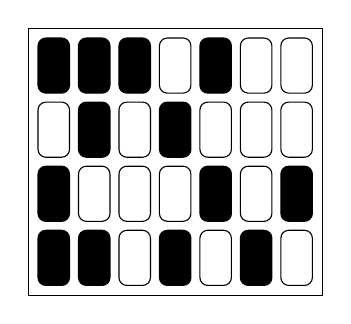
\begin{tikzpicture}[card deck]
	\matrix (m) [matrix of nodes,column sep=1mm,row sep=1mm,draw] {
	|[black card]| & |[black card]| & |[black card]| & |[white card]| & |[black card]| & |[white card]| & |[white card]| \\
	|[white card]| & |[black card]| & |[white card]| & |[black card]| & |[white card]| & |[white card]| & |[white card]| \\
	|[black card]| & |[white card]| & |[white card]| & |[white card]| & |[black card]| & |[white card]| & |[black card]| \\
	|[black card]| & |[black card]| & |[white card]| & |[black card]| & |[white card]| & |[black card]| & |[white card]| \\
	};
\end{tikzpicture}
\emph{Abb.1: Rechteck von Bob}
\medskip

% field 2
\begin{tikzpicture}[card deck]
	\matrix (m) [matrix of nodes,column sep=1mm,row sep=1mm,draw] {
	|[black card]| & |[black card]| & |[black card]| & |[white card]| & |[white card]| & |[black card]| & |[black card]| & |[black card]| \\
	|[black card]| & |[black card]| & |[black card]| & |[white card]| & |[black card]| & |[white card]| & |[white card]| & |[white card]| \\
	|[white card]| & |[black card]| & |[white card]| & |[black card]| & |[white card]| & |[white card]| & |[white card]| & |[white card]| \\
	|[black card]| & |[white card]| & |[white card]| & |[white card]| & |[black card]| & |[white card]| & |[black card]| & |[black card]| \\
	|[black card]| & |[black card]| & |[white card]| & |[black card]| & |[white card]| & |[black card]| & |[white card]| & |[white card]| \\
	};
	\begin{scope}[on background layer]
	\fill[card bg] (m.north west) -- (m.north east) -- (m.south east) -- (m-5-8.west|-m.south) -- (m-1-8.south west) -- (m.west|-m-1-1.south) -- cycle;
    \end{scope}
\end{tikzpicture}
\emph{Abb 2: Das erweiterete Rechteck}
\medskip

% field 3
\begin{tikzpicture}[card deck]
	\matrix (m) [matrix of nodes,column sep=1mm,row sep=1mm,draw] {
	|[black card]| & |[black card]| & |[black card]| & |[white card]| & |[white card]| & |[black card]| & |[black card]| & |[black card]| \\
	|[black card]| & |[black card]| & |[black card]| & |[white card]| & |[black card]| & |[white card]| & |[white card]| & |[white card]| \\
	|[white card]| & |[black card]| & |[white card]| & |[black card]| & |[white card]| & |[white card]| & |[white card]| & |[white card]| \\
	|[black card]| & |[white card]| & |[white card]| & |[white card]| & |[white card]| X & |[white card]| & |[black card]| & |[black card]| \\
	|[black card]| & |[black card]| & |[white card]| & |[black card]| & |[white card]| & |[black card]| & |[white card]| & |[white card]| \\
	};
	\begin{scope}[on background layer]
	\fill[card bg] (m.north west) -- (m.north east) -- (m.south east) -- (m-5-8.west|-m.south) -- (m-1-8.south west) -- (m.west|-m-1-1.south) -- cycle;
    \end{scope}
\end{tikzpicture}
\emph{Abb 3: Karte X wird umgedreht}
\end{wrapfigure}
\textbf{Alice, Boc und Eve machen einen Kartentrick:}

Alice legt auf einem Tisch eine bestimmte Menge von Karten mit einer schwarzen und einer weißen Seite zu einem Rechteck zusammen (zunächst liegen nur weiße Seiten oben). Nun dreht Bob einige dieser Karten um, so dass die schwarze Seite oben liegt. Das Rechteck sieht jetzt wie in Abbildung 1 aus. Eve merkt sich die Anordnung der Karten so gut sie kann und verlässt den Raum.

Alice legt nun eine weitere Reihe von Karten über das Rechteck und eine weitere Spalte rechts daneben. Nun sieht es wie in Abbildung 2 aus. \textit{Wie sie das macht, hat sie vorher mit Eve heimlich abgesprochen!}

Während Eve draußen ist, verändert Bob eine einzige Karte im Rechteck, indem er sie umdreht. Zum Beispiel die Karte X in Abbildung 3. Eve betritt wieder den Raum un erkennt sofort, welche Karte verändert wurde.

Bob staunt! Er fragt sich, wie Eve das gemacht hat.

\begin{aufgabe}[symbol=\Large\symPartner]
	Weshalb kann Eve die \enquote{falsche} Karte sofort finden, obwohl sie außerhalb des Raumes war, als die Karte umgedreht wurde? Erklärt den Trick!
	
	\tipp{Scanne den QR-Code rechts, wenn ihr einen Tipp möchtet.}
	\qrcode[height=2cm,nolink]{Hat es vielleicht etwas damit zu tun, dass Alice das Quadrat ergaenzt hat? Es hat auf jeden Fall etwas mit den schwarzen Karten zu tun.}
\end{aufgabe}

\begin{aufgabe}[symbol=\Large\symPartner]
	Eine Karte spielt eine besondere Rolle: Die Karte in der Ecke oben rechts, da sich dort die neue Reihe und die neue Spalte kreuzen. Kann diese Karte \textbf{immer passend} gelegt werden? Oder gibt es Fälle, in denen sie weiß \emph{und} schwarz sein müsste? 
	
	Probiert verschiedene Fälle mit 2x2-, 2x3- und 3x3-Rechtecken aus!
\end{aufgabe}
\end{wrapfig}

\vspace{1cm}
\begin{rahmen}\centering
	Klebe hier den Text der Zusatzaufgabe ein, die du am Pult holen kannst.
	\vspace{4cm}
\end{rahmen}

\newpage\nohead

\newsavebox{\aufgabeDrei}
\savebox{\aufgabeDrei}{%
\begin{rahmen}
	\textbf{\rmfamily\llap{\symPartner~} Aufgabe 3}\par\smallskip
	Wir ändern den Kartentrick etwas ab: Anstatt die Zeilen und Spalten so zu ergänzen, dass wir eine gerade Anzahl schwarze Karten haben, ergänzen wir sie so, dass wir jeweils eine ungerade Anzahl schwarze Karten erhalten. Ansonsten funktioniert der Trick wie bisher.
	
	Zeigt, dass es nun Fälle gibt, in denen die Karte oben rechts nicht mehr passend gelegt werden kann. In welchen Fällen funktioniert das Verfahren noch, und wann funktioniert es nich mehr?
	
	\tipp{Es hat etwas mit der Anzahl an Zeilen und Spalten zu tun.}
\end{rahmen}%
}

\usebox{\aufgabeDrei}

\vfill
\usym{2701}\dotfill
\vfill

\usebox{\aufgabeDrei}

\vfill
\usym{2701}\dotfill
\vfill

\usebox{\aufgabeDrei}

\vfill
\usym{2701}\dotfill
\vfill

\usebox{\aufgabeDrei}

\end{document}
